% !TEX encoding = UTF-8
% !TEX TS-program = pdflatex
% !TEX root = ../tesi.tex

%**************************************************************
\chapter{Configurazione dello stato iniziale}
\label{cap:configurazione-stato-iniziale}
%**************************************************************

\intro{In questo capitolo vengono descritti i procedimenti attuati per configurare lo stato iniziale dei sistemi e utilizzati.}\\

Avendo familiarità con Ubuntu ho, inizialmente, verificato che il pacchetto del server di FreeIPA fosse presente: ho presto appreso che esso era discontinuo sulle ultime versioni del sistema operativo.

Così, ho deciso di optare per CentOS Stream 9, ultima versione disponibile, per l'ottima compatibilità con FreeIPA e la migliore usabilità in ambienti server.

A questo punto, con l'aiuto del team di \myAzienda, ho configurato LXC sulla mia macchina Ubuntu 22.04 LTS. 

Tramite il comando \texttt{lxc-create -t download -n ipa-server}, ho creato un nuovo container con il nome di \emph{ipa-server} indicando di voler scaricare il template dalla lista di quelli disponibili, dalla quale ho scelto l'immagine di CentOS Stream 9 (\autoref{fig:lxc-template}).

\begin{figure}[!h] 
    \centering 
    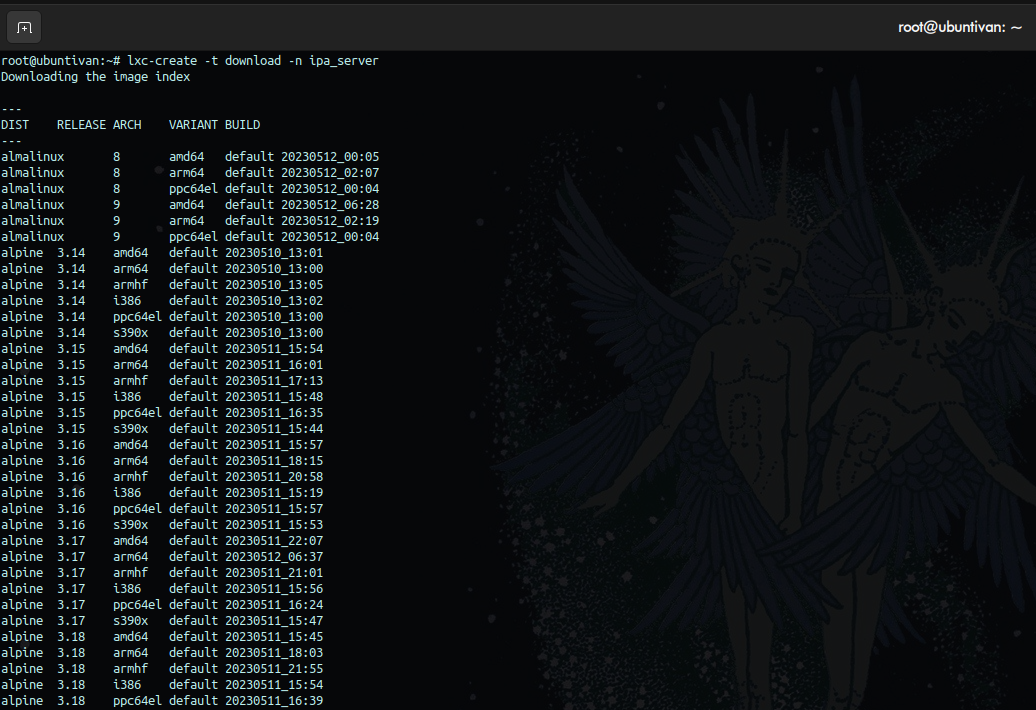
\includegraphics[width=\columnwidth]{lxc-templates} 
    \caption{Vista parziale del template download di LXC}
    \label{fig:lxc-template}
\end{figure}

Dopo la creazione della macchina ho lanciato i comandi \texttt{lxc-start ipa-server} e \texttt{lxc-console ipa-server}, rispettivamente per avviare il container e per accedere al relativo terminale.


Dopo aver configurato il container per il server ed aver eseguito l'aggiornamento dei pacchetti con il comando \texttt{yum update}, sono passato all'installazione del server di FreeIPA, disponibile su quella release con il pacchetto \emph{freeipa-server}.


Al mio arrivo negli uffici di \myAzienda, l'azienda aveva già configurato per me un account sulla loro piattaforma di testing, \emph{test.monokee.com}, utilizzando come e-mail il mio indirizzo istituzionale e garantendomi l'accesso a tutte le risorse della piattaforma, oltre che alla documentazione aziendale.